% "Станет проще"

\documentclass[a4paper,12pt]{article} % тип документа

% report, book

%  Русский язык

\usepackage[T2A]{fontenc}			% кодировка
\usepackage[utf8]{inputenc}			% кодировка исходного текста
\usepackage{graphicx}
\usepackage[english,russian]{babel}	% локализация и переносы


%отступ
\usepackage[left=3cm,right=3cm,
    top=3cm,bottom=3cm,bindingoffset=0cm]{geometry}

% Математика
\usepackage{amsmath,amsfonts,amssymb,amsthm,mathtools} 
\usepackage{csvsimple}
\usepackage{multirow}

\usepackage{hyperref}
\usepackage{wasysym}
\usepackage{subcaption}
\usepackage{verbatim}
\usepackage{hyperref}
\usepackage{float}
\usepackage{enumerate}
\usepackage[dvipsnames]{xcolor}
%Заговолок
%\graphicspath{ {images/} }


\begin{titlepage}
\author{Соловьянов Михаил }
\title{Задание 9. Электродинамика.  Протекший заряд и суммирование. Переходные процессы!}
\date{\today}
\end{titlepage}



\begin{document} % начало документа
\maketitle
http://easyfizika.ru/zadachi/elektrostatika/






\section{Контрольные вопросы}
\begin{enumerate}






\item Контрольный вопрос:
\begin{figure}[H]
\centering
  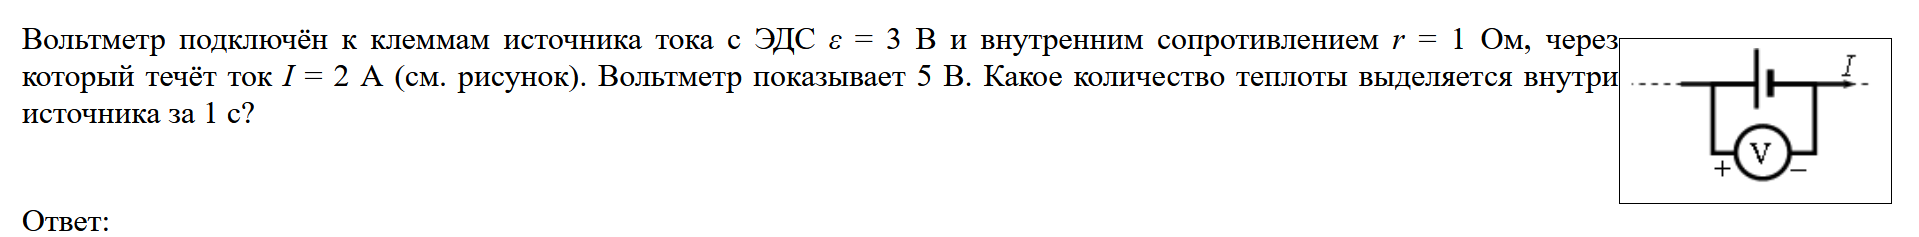
\includegraphics[width=1.1\linewidth]{KV1.PNG}
  \caption{Контрольный вопрос 3}
  \label{task0}
\end{figure}

\end{enumerate}


\section{Задачи}
\begin{enumerate}









\end{enumerate}

\section{Литература}
\begin{thebibliography}{}
    \bibitem{l1} СБОРНИК ОЛИМПИАДНЫХ ЗАДАЧ ПО ФИЗИКЕ Под редакцией Н.С. Кравченко
	
\end{thebibliography}



\end{document}